\documentclass[10pt,twoside,a4paper]{article}

% I could put all of this into a file and then \input{} it

%% PACKAGES %%
\usepackage{mathtools} % amsmath plus some fixes
\usepackage{amssymb} %symbols such as "therefore"
\usepackage{bm} % bold maths symbols
\usepackage{natbib} % for biliography and citation commands
\setcitestyle{numbers,square,comma} % see https://gking.harvard.edu/files/natnotes2.pdf

\usepackage{ulem} %underline empahsis
\usepackage{enumitem} %altering list style
\usepackage{tcolorbox}
\usepackage{listings}
\usepackage{xcolor}
\usepackage{realboxes}
\usepackage{graphicx}
\usepackage{textcomp}
\usepackage{caption}
\usepackage{colortbl}
\usepackage{hyperref}



%% PARAMETERS %%
\setlist[description]{
	style=nextline, 
%	labelwidth=0em, 
%	leftmargin=1em,
%	%itemindent=\dimexpr-5pt-\labelsep\relax, 
%	labelsep=15em,
%	labelindent=\parindent,
%	font=\normalfont
}
\definecolor{bgCodeColor}{rgb}{0.95,0.95,0.95}
\lstdefinestyle{generalCodeStyle}{
	backgroundcolor=\color{bgCodeColor},
	basicstyle=\ttfamily\small
}
\lstset{style=generalCodeStyle}
\captionsetup{justification=raggedright,singlelinecheck=false}

%% COMMANDS %%
\newcommand{\aj}{Astrophysical Journal} % command for references
\newcommand{\aap}{Astronomy and Astrophysics} % command for references

\newcommand{\sups}[1]{\textsuperscript{#1}}
\newcommand{\subs}[1]{\textsubscript{#1}}
\renewcommand{\emph}[1]{\textit{#1}}
\newcommand{\eemph}[1]{\uline{#1}}
\newcommand{\eeemph}[1]{\textbf{#1}}
\newcommand{\eeeemph}[1]{\textsc{#1}}
\newcommand{\code}[1]{\Colorbox{bgCodeColor}{\lstinline{#1}}}

\newcommand{\subsubsubsection}[1]{\smallskip \paragraph{\noindent #1}~\\}

\newcommand{\jnote}[1]{\textcolor{red}{[#1]}}

\newcommand{\tabref}[1]{Tbl.~\ref{#1}}
\newcommand{\secref}[1]{Sec.~\ref{#1}}
\newcommand{\figref}[1]{Fig.~\ref{#1}}

\newcommand{\rt}[1]{\ensuremath{\textrm{#1}}}

\newcommand{\mat}[1]{\ensuremath{\bm{#1}}} % how we are showing a matrix
\renewcommand{\vec}[1]{\ensuremath{\underline{#1}}} % how we are showing a vector
\newcommand{\tr}[1]{\ensuremath{#1^{\rt{T}}}} % transpose operation for a vector/matrix
\newcommand{\inv}[1]{\ensuremath{#1^{-1}}} % inverse operation for a scalar/vector/matrix
\newcommand{\abs}[1]{\ensuremath{\left|{#1}\right|}} %magnitude operator
\newcommand{\partialdiff}[2]{\ensuremath{\frac{\partial #1}{\partial #2}}} %partial differential
\newcommand{\ppartialdiff}[2]{\ensuremath{\frac{\partial}{\partial #2}\left[ #1 \right]}} %partial differential, prefix version
\newcommand{\partialddiff}[2]{\ensuremath{\frac{\partial^{2} #1}{\partial #2^{2}}}} %partial differential
\newcommand{\ppartialddiff}[2]{\ensuremath{\frac{\partial^{2}}{\partial #2^{2}}\left[ #1 \right]}} %partial differential, prefix version

\newcommand{\rarrow}{\ensuremath{\rightarrow}}

% Fourier transform commands
\newcommand{\fft}[1]{\ensuremath{\mathcal{F}\left[ #1 \right]}}
\newcommand{\fftconj}[1]{\ensuremath{\mathcal{F}^{*}\left[ #1 \right]}}
\newcommand{\ifft}[1]{\ensuremath{\mathcal{F}^{-1}\left[ #1 \right]}}
\newcommand{\ifftconj}[1]{\ensuremath{{\mathcal{F}^*}^{-1}\left[ #1 \right]}}

% text mode commands
\renewcommand{\_}{\textunderscore\linebreak[0]}
\newcommand{\la}{\textlangle}
\newcommand{\ra}{\textrangle}


% LOCAL COMMANDS %
\newcommand{\trp}[1]{\ensuremath{\left(#1\right)^{\rt{T}}}}
\newcommand {\y} {\vec{y}}
\newcommand {\ym} {\vec{y}_m}
\newcommand {\yc} {\vec{y}_0}
\newcommand {\ye} {\hat{\vec{y}}}
\newcommand {\K} {\mat{K}}
\renewcommand{\k} {\vec{k}}
\newcommand {\x} {\vec{x}}
\newcommand {\xe} {\hat{\vec{x}}}
\newcommand {\xc} {\vec{x}_0}
\newcommand {\xa} {\vec{x}_a}
\renewcommand {\L} {\mat{L}}
\newcommand {\La} {\mat{L}_a}
\newcommand {\rb}[1]{\left(#1\right)}
\renewcommand {\sb}[1]{\left[#1\right]}
\newcommand {\Sm} {\mat{S}_m}
\newcommand {\Sa} {\mat{S}_a}

% ENVIRONMENTS %
\newenvironment{aside}
{ 
	\hfill\break
	\begin{tcolorbox}
}
{
	\hfill\break
	\end{tcolorbox}
}

\begin{document}
	\title{Deconvolution Tutorial}
	\author{Dr. Jack Dobinson}
	\date{\today}
	\maketitle

	\begin{abstract}
	Notes on the decovolution routines I've created. I've copied the relevant parts of my code-base into the `scripts' folder. All the main routines are in the `./scripts/fitscube/deconvolve/' sub-folder. Each of the `./tutorial*/' folders contains an example implementation of one of the main routines I've used. Hopefully they should all run if you use the command \code{python3 -I ./run_XXX.py} from inside the folder.
	\end{abstract}
	
	\section{Python Setup}
		\label{sec:python_setup}
		
\subsection{Useful Information}
\begin{description}
	\item{Version\\} Python 3.9.6 ($\geq$ 3.8 required)
	\item{3rd Party Packages (used for the tutorials)}
		\begin{description}
			\item{numpy\\} \verb|https://numpy.org/install/|
			\item{scipy\\} \verb|https://scipy.org/install/|
			\item{matplotlib\\} \verb|https://matplotlib.org/stable/users/getting_started/|
			\item{astropy\\} \verb|https://docs.astropy.org/en/stable/install.html|
		\end{description}
	\item{Virtual Environments}
	\begin{description}
		\item{pyenv\\} \verb|https://github.com/pyenv/pyenv| Used to manage multiple versions of python without interfering with the system's installation. See this tutorial for details \texttt{https://towardsdatascience.com/managing-\linebreak[0]virtual-\linebreak[0]environment-\linebreak[0]with-\linebreak[0]pyenv-\linebreak[0]ae6f3fb835f8}
		\item{virtualenv\\} \verb|https://github.com/pyenv/pyenv-virtualenv| A plugin for pyenv to manage multiple virtual environments
		\item{anaconda\\} \verb|https://www.anaconda.com/products/distribution| A managed distribution and virtual environment manager. I've not used it really, but lots of people like it.
	\end{description}
	
\end{description} 



\subsection{Background}

Updating and upgrading Python and it's packages can be a horrible can of worms. The main problem is that many computers come with a \emph{system} installation of Python. The \emph{system} installation is required, as some utilities and system-level things need it. Unfortunately, if you update to a newer version of Python (especially if you swap your `python` command to point to a `python3` executable) nasty things can happen. Therefore, rather than solving the problem people stuck a patch on it called \emph{version managers}, \emph{virtual environments}, and \emph{virtual environment managers}.

Technically, you can install a different version of Python onto your system just by providing some variables when installing it. However, it can become a massive hassle to rememeber which versions you need and where you kept them. `pyenv' is a version manager, and can let you replace the commands `python' and `python3' with whatever you want without interfering with the \emph{system} installation. I've managed to set up `pyenv' on my machine such that I never have to do anything special unless I'm updating to a new version of python (and then I just need to change the `global' version to the new one and ignore it again).

A virtual environment, just swaps out all of the environment variables that Python needs to different versions so they don't interfere with the \emph{system} installation or any other installation. This is useful if you need a specific version of a package (to run some archaic scripts you found), but that version is incompatible with your normal setup. `pyenv' has a plugin called `pyenv-virtualenv' that can make and manage virtual environments for you.

Anaconda is a managed python distribution that comes with a version manager and virtual environment manager built-in. I've not used it much, but many people do and it's considered good. It's probably the simplest way to get everything working, they also have a `miniconda' version that just installs their management software so you can customise everything yourself.





	\section{Deconvolution}
		\label{sec:deconvolution}
		

\subsection{Notation}
	\begin{description}
		\item{$O(\x)$} The \emph{ground truth} signal (true-signal, or original-signal), i.e. what we would measure if our instruments were perfect.
		\item{$R(\x)$} The response function of an instrument. Usually called the Point Spread Function (PSF) when talking about telescopes.
		\item{$N(\x)$} Some noise function that corrupts $O(\x)$.
		\item{$I(\x)$} The observational data recorded by the instrument. I.e., $O(\x)$ after it has been passed through the response function and corrupted by noise.
		\item{$\x$} A vector that holds the state of a system, in our case $\x$ is the position of a pixel in an image.
		\item{$\fft{...}(u)$} The fourier transform operation to some conjugate space denoted by $u$.
		\item{$\ifft{...}(x)$} The inverse fourier transform back to the original space denoted by $x$.
		\item{$\tilde{\square}$} An estimate of the decorated symbol.
		\item{$\square^\star$} Conjugate transpose of the decorated symbol.

	\end{description}		

\subsection{PSF Normalisation}
In the rest of this document, I've made the implicit assumption that the Response Function, $R(\x)$ (or PSF for telescopes), is normalised. By that, I mean the following conditions are true:
\begin{itemize}
	\item $\sum_{\x} R(\x) = 1$, I.e. convolving (or deconvolving) the observation with the response function does not change the total sum of the signal, except for edge effects in some cases.
	\item If $R(\x)$ is represented as a vector or array, it's shape is \emph{odd} in all of it's dimensions. I.e. A PSF needs to have a unambiguous central pixel.
	\item $R(\x)$ is centered such that convolution (or deconvolution) with $R(\x)$ does not shift a signal. I.e. A PSF's centroid (and hopefully brightest pixel) is coincident with it's central pixel. Hence the need for an unambiguous center.
	\item $R(\x)$ Has no NANs in it, generally these play havok with convolution and deconvolution routines.
\end{itemize}
	
A failure of these conditions can typically be fixed after the fact (except for the NAN condition) by working out what the effect was and undoing it, but it's a hassle.

\subsection{Background}

For any original signal, $O(\x)$, measured by an instrument there is some corruption due to non-perfect response $R(\x)$, and noise $N(\x)$, which gives an observation $I(\x)$ that is related to the original signal by
\begin{align}
	I(\x) 	&= \int {R(\x-\x_1) \, O(\x_1)} \, d\x_1 + N(\x) \nonumber \\
			&= (R \star O)(\x) + N(\x)
	\label{eq:convolution}
\end{align}
where $\star$ denotes the convolution operation.

The problem we face much of the time is recovering the original signal $O(\x)$ from the observed data $I(\x)$ as accurately and quickly as possible.

The convolution theorem
\begin{align}
	\fft{(f \star g)(x)}(k) = \fft{f(x)}(k) \fft{g(x)}(k),
	\label{eq:conv_theorem}
\end{align}
where $\fft{f(x)}(k)$ denotes the fourier transform of $f(x)$, $k$ is the conjugate variable to $x$, and $\ifft{...}(x)$ denotes the inverse fourier transform operation, helps us see some way to fix the problem.

As the Fourier transform is a linear operator,
\[
	\fft{I(\x)}(\vec{k}) = \fft{R(\x)}(\vec{k}) \, \fft{O(\x)}(\vec{k}) 
							+ \fft{N(\x)}(\vec{k}),
\]
which can be re-arranged to give
\begin{align}
	\fft{O(\x)}(\k) &= \frac{\fft{I(\x)}(\k) - \fft{N(\x)}(\k)}
						{\fft{R(\x)}(\k)},
	\label{eq:fourier_quotient}
\end{align}
the \emph{fourier quotient} method of deconvolution. Unfortunately in practice there is a frequency cutoff to our measurements of $R(\x)$ and close to that cutoff the noise $N(\x)$ is amplified, leaving \eqref{eq:fourier_quotient} unusable where there is any high-frequency noise, which there usually is.

Also, \eqref{eq:convolution} is typically an ill-posed problem as there are many possible $O(\x)$ functions that can give a $I(\x)$ observation. Therefore, deconvolution in general is used to find a method which gives an \emph{estimate}, $\tilde{O}(\x)$, of the original signal.


\subsubsection{Lucy-Richardson}

Many approaches to deconvolution take inspiration from fitting algorithms and probability theory; one widely used method is Lucy-Richardson (LR) \cite{Richardson72,Lucy74} deconvolution \cite[][section 5.4]{Starck02}. LR-deconvolution is based on the principle of finding a maximum likelihood estimator (MLE) for $O(\x)$

The likelyhood comes from Bayes theorem
\begin{align}
	p(O|I) = \frac{p(I|O) p(O)}{p(I)},
	\label{eq:bayes_theorem}
\end{align}
where $p(O|I)$, the likelyhood, is the probability that our estimate $\tilde{O}(\x)$ is the original signal $O(\x)$ for some observed data $I(\x)$, $p(I|O)$ is the probability that we could get our observed data $I(\x)$ from our estimate $\tilde{O}(\x)$, $p(O)$ is the probability our estimate is correct, and $p(I)$ is the probability our data is correct.

When minimising \eqref{eq:bayes_theorem}, our observational data $I(\x)$ is constant, and $O(\x)$ is the subject. Therefore $p(I)$ will not change, but $p(I|O)$ will vary depending on the different original signals we test. $p(I|O)$ is the probability of getting our observed data $I(\x)$ from some original signal $O(\x)$, i.e. it is the joint probability that, given some statistical model $\mathcal{N}$ we would draw $I(\x)$ from the possible set of functions given by $(R\star O)(\x)$, i.e.

\begin{align*}
	p(I|O) 	&= \prod_{\x} (\mathcal{N}[(R \star O)(\x)] = I(\x)) \\
			&= \prod_{\x} f_{\mathcal{N}}(I(\x);(R \star O)(\x))
\end{align*}
Or, as this is always positive we can use the log-likelihood instead
\begin{align}
	l(O|I) &= \textrm{ln}[\mathcal{L}(O|I)] = ln[p(I|O)] \nonumber \\
		&= \sum_{\x} \textrm{ln}[f_{\mathcal{N}}(I(\x);(R \star O)(\x)] \\
	\label{eq:likelihood}
\end{align}
where $f_{\mathcal{N}}(a(\x); \theta(\x))$ is the probability mass function (or probability density function for continuous distributions) for a random variable to be $a(\x)$ when it is drawn from the distribution $\mathcal{N}$ with the parameters $\theta(\x)$, $\mathcal{L}(O|I)$ is the \emph{likelihood} of $O(\x)$ given we have the data $I(\x)$, and $l(O|I)$ is the \emph{log-likelihood}.

Since in Astronomy, images are made up of photons collected by a telescope and deposited on a CCD Poisson statisticis apply. Therefore
\begin{align*}
	\mathcal{N} &\sim \textrm{Poisson}((R \star O)(\x)) \\
	f_{\mathcal{N}}(k; \lambda) &= \frac{\lambda^{k} e^{-\lambda}}{k!} \\
	\mathcal{L}(O|I) &= \prod_{\x} \frac{(R \star O)(\x)^{I(\x)} e^{-(R \star O)(\x)}} {I(\x)!} \\
	l(O|I) &= \sum_{\x} I(\x) \textrm{ln}[(R \star O)(\x)] -(R \star O)(\x) - I(\x)!,
\end{align*}
after some manipulation \cite{LR_derivation}, we get
\begin{align}
	O_{n+1}(\x) = \left[\frac{I}{\left( R \star O_n \right)} \star R^\star \right](\x) \, O_n(\x)
	\label{eq:lr_deconv}
\end{align}
where successive iterations give new approximations to the original signal. 

In general LR-deconvolution works well for point-like sources, however where to stop the iteration is non-trivial. As $n$ increases, higher and higher fourier frequencies are being deconvolved and you start running into the same problem as \eqref{eq:fourier_quotient}, noise becomes amplified.

\subsubsection{Modified CLEAN}

CLEAN \cite{hogbom74} is used extensively in radio astronomy, and occasionally in the wider astronomy community \cite{Keel91}. The original algorithm builds up an estimate $\tilde{O}(\x)$ (the \emph{component map}) by subtracting the response function convolved with low-amplitude delta-functions from $I(\x)$, and adding them to the estimate. I.e.
\begin{align}
	\tilde{O}_0(\x) &= \vec{0} \nonumber \\
	I_n(\x) &= I(\x) - (R \star \tilde{O}_n)(\x) \nonumber \\
	x_i &= \textrm{argmax}[I_n(\x)] \nonumber \\
	\tilde{O}_{n+1}(\x) &= \tilde{O}_n(\x) + g_\textrm{loop} I_n(x_i)
	\label{eq:hogbom_clean}
\end{align}
where $g_\textrm{loop}$ is the \emph{loop-gain}, the fraction of the brightest pixel added to the \emph{components}, $\tilde{O}(\x)$, each iteration. Stopping criteria are fairly standard, usually once $I_n(x_i)$ has reduced by some factor. Once the component map $\tilde{O}(\x)$ is complete, it is convolved with the \emph{clean beam} $\tilde{R}(\x)$, a response function that does not have the wings of the original $R(\x)$ (the \emph{dirty beam}) this gives the \emph{clean map} $\tilde{I}(\x) = (\tilde{R} \star \tilde{O})(\x)$.

This method has various problems for our purposes, mostly that extended sources are not deconvolved efficiently and exhibit striping artifacts on the size scale of $R(\x)$. To get around this limitation various methods have been proposed \cite{Giovannelli21, Choi17, Wakker88, Cornwell08, Cornwell83}, for our purposes Modified CLEAN \cite{Steer84} seems to have the best properties.

Modified CLEAN works similarly to \eqref{eq:hogbom_clean} except that instead of just selecting the brightest pixel, all pixels above the selection threshold, $t_s$, are treated as a single extended source. For sufficiently small values of $g_\textrm{loop}$ and $t_s$ the subtractions will be linear enough that the differences between regions of slightly different brightness do not matter. Modified clean has the following main iterative scheme:
\begin{align}
	\tilde{O}_0(\x) &= \vec{0}, \nonumber \\
	I_n(\x) &= I(\x) - (R \star \tilde{O}_n)(\x), \nonumber \\
	\x_s &= \left\lbrace x_i; I_n(x_i) > t_s; x_i \in \x \right\rbrace , \nonumber \\
	\tilde{O}_{n+1}(\x) &= \tilde{O}_n(\x) + g_\textrm{loop} I_n(x_s).
	\label{eq:modified_clean}
\end{align}



\subsubsubsection{Variable Threshold}
Another modification to \eqref{eq:modified_clean} is to vary $t_s$, the selection threshold, to attempt to deconvolve small and bright features before more extended features.

One method is Otsu Thresholding \cite{Otsu79,otsu_thresholding}, a technique that divides a set into two different classes by choosing a dividing threshold, $t_\textrm{otsu}$, in such a way that the variance between the two classes is minimised. Apply successive Otsu thresholds to an image, and then selecting the candidate threshold that is the most \emph{exclusive} (i.e. the threshold that rejects the largest fraction of pixels per fraction of range.
\[
	e(t) = \frac{f_\textrm{range}(t) - f_\textrm{pix}(t)}{f_\textrm{range}(t) + f_\textrm{pix}(t)} ,
	\label{eq:exclusivity}
\]
where $e(t)$ is the exclusivity of a threshold $t$, $f_\textrm{range}(t) = (t - \textrm{min})/(\textrm{min} - \textrm{max})$ is the fraction of range rejected by a threshold, and $f_\textrm{pix}(t) = N_\textrm{bright}/N$ is the fraction of pixels kept by the threshold. Here $N_\textrm{bright}$ is the number of pixels above the threshold, and $N$ is the original number of pixels. Finally, $t_s$ is calculated via:
\begin{align*}
	t_{\textrm{otsu},j} &= \textrm{The j\sups{th} Otsu threshold of our image data}\,, I(\x), \\
	t_\textrm{factor} &= \textrm{A user supplied factor}\,, >0, <1, \\
	i &= \textrm{argmax}\lbrace e(t_{\textrm{otsu},j}); 0 <= j <= N_\textrm{thresholds} \rbrace, \\
	t_i &= t_{\textrm{otsu},i}, \\
	t_s &= \textrm{max}[I_n(\x)] t_\textrm{factor} + (1 - t_\textrm{factor}) t_i.
\end{align*}

As before, the final estimate of the original signal $\tilde{O}(\x)$ is normally convolved with a \emph{clean beam} $\tilde{R}(\x)$ found from the main lobe of the response function (usually an approximate gaussian) to give the \emph{clean map},
\[
	\tilde{I}(\x) = (\tilde{R} \star \tilde{O})(\x).
\]
When the components $\tilde{O}(\x)$ of the image are not well correlated with their neighbours this process can result in huge gains. However, in various tests it has been found that this step is not always neccesary for the production of a smooth image. Infact using the components directly has been better in many cases, with the extra convolution step just degrading the spatial resolution of the map.


\subsubsubsection{Flux Loss}
Typically deconvolution does not change the total sum of an observation, or any differences are marginal. However if not enough iterations are performed to completely explain all of the signal in our observation, then some difference in $\sum_{\x} I(\x)$ vs $\sum_{\x} \tilde{O}(\x)$ may occur.

The simplest way to deal with this difference is to add back the residual such that the \emph{clean map} is 
\[
\tilde{I}(\x) = (\tilde{R} \star \tilde{O})(\x) + \left[ I(\x) - (R \star \tilde{O})(\x) \right],
\]
i.e., the residual of the deconvolution is added to the output.



\subsection{Usage of \texttt{./tutorial{\textunderscore}0{\textunderscore}deconv/run{\textunderscore}deconv.py}}

\begingroup
\small
\begin{verbatim}
usage: run_deconv.py [-h] [--output.file str] [--output.file.overwrite]
                     [--CleanModified.show_plots] [--CleanModified.save_plots]
                     [--CleanModified.plot_dir str] [--CleanModified.verbose int]
                     [--CleanModified.n_iter int] [--CleanModified.loop_gain float]
                     [--CleanModified.threshold float]
                     [--CleanModified.n_positive_iter int]
                     [--CleanModified.noise_std float]
                     [--CleanModified.rms_frac_threshold float]
                     [--CleanModified.fabs_frac_threshold float]
                     OBS_FITS_PATH PSF_FITS_PATH

# DESCRIPTION #
        Front-end to deconvolution routines.

        ## Example ##
                $ python3 ./deconv.py ../data/test_rebin.fits{1}[229:230] 
                      ../data/test_standard_star.fits{1}

        ## FITS File Path Format ##
                ../path/to/datafile.fits{ext}[slice_tuple](img_axes_tuple)
                        ext : int | str
                                Extension of the FITS file to operate upon, if not present,
                                will use the first extension that has some data.
                        slice_tuple : tuple[Slice,...]
                                Slice of the data to operate upon, useful for choosing
                                a subset of wavelength channels. If not present, will
                                assume all wavelengths are to be deconvolved.
                        img_axes_tuple : tuple[int,...]
                                Tuple of the spatial axes indices, uses FITS ordering
                                if +ve, numpy ordering if -ve. Usually the RA,DEC axes.

                ### Examples ###
                        ./some_datafile.fits{PRIMARY}[100:150]
                                Select the extension called 'PRIMARY' and deconvolve the 
                                channels 100->150
                        /an/absolute/path/to/this_data.fits[99:700:50]
                                Try to guess the extension to use, deconvolve every 50th 
                                channel in the range 99->700
                        ./deconv/whole/file.fits{SCI}
                                Use the extension 'SCI'
                        ./some/path/big_file.fits{1}[5:500:10](0,2)
                                use the 1st extension (not the 0th), deconvolve every 10th 
                                channel in the range 5->500, the spatial axes are 0th and 
                                2nd axis.


# END DESCRIPTION #

positional arguments:
  OBS_FITS_PATH         Observation file to operate upon, uses FITS file path format
  PSF_FITS_PATH         Point Spread Function (PSF) to use during deconvolution, uses FITS
                        file path format

optional arguments:
  -h, --help            show this help message and exit
  --output.file str     file to output deconvolved data to. (default: ./output/deconv.fits)
  --output.file.overwrite, --output.file.no_overwrite
                        Should we overwrite the output file or not? (default: True)

CleanModified:
  
        A modified verison of the CLEAN algorithm, designed to account for non-point 
        objects better than standard CLEAN see 
        https://articles.adsabs.harvard.edu/pdf/1984A%26A...137..159S
  
        Creation of the class sets up the attributes that define how the algorithm behaves,
        calling the class runs the algorithm on input data.
  

  --CleanModified.show_plots, --CleanModified.no_show_plots
                         should plots be displayed interactively when running?
                         (default: False)
  --CleanModified.save_plots, --CleanModified.no_save_plots
                         should plots be saved to a file?
                         (default: False)
  --CleanModified.plot_dir str
                         folder to save plots to (if they should be saved), relative to
                         current working directory
                         (default: ./plots)
  --CleanModified.verbose int
                         verbosity of messages from algorithm
                         (default: 1)
  --CleanModified.n_iter int
                         Number of iterations
                         (default: 1000)
  --CleanModified.loop_gain float
                         Fraction of emission that could be accounted for by a PSF added to
                         components each iteration. Higher values are faster, but unstable.
                         I may want a way to scale this with the number of iterations, or
                         with the amount of point-like sources found each step. Once the 
                         image becomes noisy (i.e. is already noisy, or only noise left in 
                         map), this can lead to stippling accross the image when it's too 
                         high
                         (default: 0.5)
  --CleanModified.threshold float
                         Fraction of maximum brightness above which pixels will be included
                         in CLEAN step (want 0 < x < 1)
                         Some magic numbers are:
                                0
                                        Uses "otsu thresholding" to guess a good value
                                0 > x > -1
                                        Uses multiple "otsu thresholds" each iteration to
                                        get a value, and then applies the threshold value 
                                        so that higher order otsu threholds result in a 
                                        much larger effective "self.threshold" value. 
                                        Useful for deconvolving bright features on a 
                                        surface first.
                                -1
                                        Uses multiple "otsu thresholds" each iteration, 
                                        chooses a higher order one based onhow many pixels 
                                        the higher order threshold rejects. Selects for 
                                        many pixels rejected as this should mean that 
                                        small-but-bright features are deconvolved first.
                                -2
                                        Uses "otsu thresholding" each iteration, just uses 
                                        the first value.
                         (default: -1)
  --CleanModified.n_positive_iter int
                         Number of iterations to do that only "adds" emission, before 
                         switching to "adding and subtracting" emission
                         (default: 0)
  --CleanModified.noise_std float
                         Estimate of the deviation of the noise present in the observation
                         (default: 0.01)
  --CleanModified.rms_frac_threshold float
                         Fraction of original RMS of residual at which iteration is stopped
                         (default: 0.01)
  --CleanModified.fabs_frac_threshold float
                         Fraction of original Absolute Brightest Pixel of residual at which 
                         iteration is stopped
                         (default: 0.01)

END OF USAGE
\end{verbatim}
\endgroup
























































	\section{SSA Filtering}
		\label{sec:ssa_filtering}
		\subsection{Background}
	Singular Spectrum Analysis (SSA) \cite{Ghil02} was originally developed as a model-free technique to decompose a time series (including a non-stationary time series) into the sum of interpretable componets such as trend, periodic components, and noise, with no a-priori assumptions about the form of those components. For a full derivation of the 2D treatment, see \cite{Golyandina13} however the 1D form is fairly straight forward and has the same basic steps.

\subsection{Why go to the trouble?}
The problem I was trying to solve when I started using this technique was this: How can I reduce/flag instrumental artifacts that vary in position and intesity between wavelength channels without laboriously going through each image? I tried a few different techniques.

Low pass filtering had quite a few problems. It did reduce smaller artifacts, but did not affect larger ones that are extended in one dimension but not another. Furthermore, it mostly just blurred the observational data which is the exact opposite of what we are trying to achive with the whole process, namely removing blur to get good estimates of limb-darkening parameters.

Edge detection via different methods (e.g. Sobel filtering) was moderately successful, however all the techniques I found preferentially find edges along certain directions. That wasn't too much of a problem, as the routines are cheap (computationally) and can be run multiple times, but they also missed obvious artifacts and flagged non-artifact. I.e., their false positive and false negative rate are quite high.

I had a look into computer vision libraries to see if I could use motion estimation techniques like Optical Flow or Block Matching, as many artifacts move across the imaged field w.r.t.~wavelength. However, this had a couple of problems. One, not all of the artifacts move and I would still have to find some way to deal with them. Two, I was starting to veer into having to learn a lot about computer vision which was probably just as much work as going through the images manually (at least for one observation).

SSA was suggested to me by a friend, and while it is certainly not perfect, it has a good balance of flagging obvious artifacts, not flagging actual data, and being fairly computationally efficient. In the implementation I'm using it's not using any wavelength-varying information, so there's probably a way to improve it (3D SSA?) or use a secondary technique to identify artifacts that move with wavelength.

\subsubsection{Singular Value Decomposition}
SSA uses Singular Value Decomposition (SVD) to split up a series into components, here's a quick overview of it. SVD factorises an $m \times n$ matrix into an orthogonal eigenbasis.

\[
	\mat{M} = \mat{U}\mat{\Sigma}\mat{V}^\star
\]
\begin{center}
\begin{tabular}{l|l}
 Matrix 			& Shape  			\\
 \hline	
 $\mat{M}$ 		& $(m \times n)$ 	\\
 $\mat{U}$ 		& $(m \times m)$ 	\\
 $\mat{\Sigma}$ 	& $(m \times n)$   	\\
 $\mat{V}$ 		& $(n \times n)$ 
\end{tabular}
\end{center}

$\mat{M}$ is the matrix to factorise, $\mat{U}$ is the left singular matrix, $\mat{\Sigma}$ holds the singular values along its diagonal, and $\mat{V}$ is the right singular matrix. $\mat{U}$ and $\mat{V}$ are \emph{unitary}, their conjugate transpose is their inverse, and $\mat{\Sigma}$ is a diagonal matrix with non-negative real numbers on its diagonal.

SVD gives a non-unique solution, however we can always choose $\Sigma_{ii}$'s to be in decending order. In which case $\mat{\Sigma}$ is unique, but $\mat{U}$ and $\mat{V}$ are not.

Sometimes the compact form of SVD is used, which only includes the non-zero terms in $\mat{\Sigma}$, in this case the shapes of the matrices are changes such that $\mat{U}$ is shape $(m \times r)$, $\mat{\Sigma}$ is shape $(r \times r)$, and $\mat{V}$ is shape $(r \times n)$. In this case $\mat{U}$ and $\mat{V}$ are \emph{semi unitary}, and $r$ is the number of non-zero elements in the original $\mat{\sigma}$.


\subsubsection{Method}
Let $\mat{\mathbb{X}}$ be a real-values time series, $\mat{\mathbb{X}} = (x_1, x_2, ..., x_n)$ of length $N$, let $L$ (with $1<L<N$) be an integer called the \emph{window length}, and $K = N - L + 1$.

First form the \emph{trajectory matrix} $\mat{X}$, the $L \times K$ matrix that holds each moving window of length L in its columns.
\[
	\mat{X} = \begin{pmatrix}
	x_1 & x_2 & ... & x_K \\
	x_2 & x_3 & ... & x_{K+1} \\
	\vdots & \vdots & \ddots & \vdots \\
	x_L & x_{L+1} & ... & x_{N} 
	\end{pmatrix}
\]
$\mat{X}$ is a \emph{Hankel} matrix, i.e., all its anti-diagonals have constant elements.

Secondly, perform SVD on $\mat{X}$. A slightly faster way than the direct version is the following. Compute
\begin{align*}
	\mat{S} &= \mat{X}\mat{X}^\textrm{T},
\end{align*}
S is of shape $L \times L$, and let $\lambda_1, \lambda_2,...,\lambda_L$ be the \emph{eigenvalues} of $\mat{S}$. Therefore,
\begin{align*}
	\mat{S} &= (\mat{U}\mat{\Sigma}\mat{V}^\star)(\mat{U}\mat{\Sigma}\mat{V}^\star)^\star \\
		&= \mat{U}\mat{\Sigma}\mat{V}^\star\mat{V}\mat{\Sigma}^\star\mat{U}^\star \\
		&= \mat{U}\mat{\Sigma}^2\mat{U}
\end{align*}
the eigenvalues of $\mat{S}$ are the squares of the singular values of $\mat{X}$, and the eigenvectors of $\mat{S}$ are the columns of the left singular matrix $\mat{U}$ of $\mat{X}$. Also,
\begin{align*}
	\mat{X}^\star &= \mat{V} \mat{\Sigma}^\star \mat{U}^\star \\
	\rightarrow \quad \mat{X}^\star \mat{U} \mat{\Sigma}^{-1} &= \mat{V} 
\end{align*}
means that the right singular matrices $\mat{V}$ of $\mat{X}$ can be found via
\begin{align*}
	V_i = \frac{\mat{X}^\star \mat{U}}{\sqrt{\lambda_i}}.
\end{align*}

So, the SVD can be decomposed into a sum via
\begin{align*}
	\mat{U} &= (U_1, U_2, ..., U_L) \\
	\mat{V} &= (V_1, V_2, ..., V_K) \\
	\textrm{let} \quad d &= \textrm{min}(L,K) \\
	\mat{X} &= (U_1, U_2, ..., U_L) \mat{\Sigma} (V_1, V_2, ..., V_K)^\star \\
			&= (U_1 \Sigma_{11}, U_2 \Sigma_{22}, ..., U_d \Sigma_{dd}) (V_1, V_2, ..., V_d)^\star \\
			&= \sum_{i=1}^{d} \Sigma_{ii} U_i V_i^\star
\end{align*}
such that
\begin{align*}
	\mat{X} &= \mat{X}_1 + \mat{X}_2 + ... + \mat{X}_d \\
	\mat{X}_i &= \sqrt{\lambda_i}U_iV_i^\star.
\end{align*}
The $(\sqrt{\lambda_i}, U_i, V_i)$ quantities are the \emph{eigentriples} of the SVD of $\mat{x}$. Sometimes $\sqrt{\lambda_i}V_i$ are called the \emph{principle components} of $\mat{X}$. $\mat{X}_i$'s are called the \emph{elementary matrices}.

Thirdly, group the eigentriples. This step is kinda optional, you can just use the elementary matrices directly, called \emph{elementary grouping}, but inspecting the eigentriples and grouping together those whose singular vectors vary at a similar frequency can reveal trends and periodic components to the data. 

In maths terms, partition the indices $\lbrace 1, 2, ..., d\rbrace$ into $l$ disjoint subsets $I_1, I_2, ..., I_l$, with $I = \lbrace 1,2,...,p \rbrace$. Therefore $\mat{X}_I$ corresponding to group $I$ is $\mat{X}_I = \mat{X}_{i_1} + \mat{X}_{i_2} + ... + \mat{X}_{i_p}$, and
\[
	\mat{X} = \mat{X}_{I_1} + \mat{X}_{I_2} + ... + \mat{X}_{I_l}
\]

Fourth, diagonally average the grouped matrices and extract the associated time-series. Each $\mat{X}_{I_j}$ matrix is \emph{Hankelised} (i.e., their anti-diagonals are averaged), and the time-series associated with hankelised matrix $\tilde{\mat{X}}_{I_j}$ is extracted by takling the main diagonal to get a reconstructed time series
\[
	\tilde{\mat{\mathbb{X}}}^{(j)} = (\tilde{x}_1^{(1)}, \tilde{x}_2^{(2)}, ...,\tilde{x}_N^{(N)}). 
\]
Therefore, the initial series $\mat{\mathbb{X}} = (x_1, x_2, ..., x_n)$ is decomposed into a sum of $l$ reconstructed subseries
\begin{align*}
	x_n &= \sum_j^{l} \tilde{x}_n^{(j)}, \quad \textrm{where} \quad n \in (1,2,...,N) \\
	\textrm{such that}& \\
	\mat{\mathbb{X}} &= \tilde{\mat{\mathbb{X}}}^{(1)} + \tilde{\mat{\mathbb{X}}}^{(2)} + ... + \tilde{\mat{\mathbb{X}}}^{(l)}.
\end{align*}

\begin{aside}
	Hankelisation is the process of taking some matrix $\mat{A}$ and replacing each anti-diagonal with the mean of the elements on that diagonal. E.g.
	\begin{align*}
		\mat{A} = \begin{pmatrix}
			a_1 & a_2 & a_3 \\
			a_4 & a_5 & a_6 \\
			a_7 & a_8 & a_9 
		\end{pmatrix} 
		\quad \rightarrow \quad	
		\tilde{\mat{A}} &= \begin{pmatrix}
			\tilde{a_1} & \tilde{a_2} & \tilde{a_3} \\
			\tilde{a_2} & \tilde{a_3} & \tilde{a_4} \\
			\tilde{a_3} & \tilde{a_4} & \tilde{a_5}
		\end{pmatrix}.
	\end{align*}


	In general for an $m \times n$ matrix,
	\begin{align*}
		\tilde{a_k} =& \frac{ \sum\limits_{(i,j) \in D_k} a_{ij} }{\textrm{Count}(D_k)} \\
		D_k =& \lbrace (i,j) : i+j = k+1, 1 \leq i \leq m, 1 \leq j \leq n \rbrace \\
		\textrm{Count}(D_k) \coloneqq & \textrm{The number of elements in $D_k$}
	\end{align*}
\end{aside}

To summarise, window length $L$ determins the resolution of the SSA, larger $L$ captures more data and therefore leads to better separability of different components. Also, $L$ defines the largest periodic features that can be captured. Trends are found by grouping eigentriples with slowly varying eigenvalues, periodicity is found by grouping similarly sized eigenvalues with periodically varying eigenvectors, noise is generally small (but not always) eigenvalues with stochastically varying eigenvectors.

Applying SSA to an image instead of a time series uses 2D-SSA \cite{Golyandina13}. In image space, instead of trends over time, you are looking at variation over space. The $\tilde{\mat{\mathbb{X}}}^{(j)}$ decomposed images therefore show decomposed spatial trends, periodicity, and noise.

In the SSA filtering routine, I've implicity assumed that noise is separated into components with smaller eigenvalues. For each decomposed image, $\tilde{\mat{\mathbb{X}}}^{(j)}$, the cumulative distribution function $p(\tilde{x}_i^{(j)} \leq x; \tilde{x}_i^{(j)} \in \tilde{\mathbb{X}}^{(j)}) $ is calculated, and then transformed to give each pixel a score $s_i^{(j)}$ via
\[
	s_i^{(j)} = 4(p(\tilde{x}_i^{(j)} \leq x; \tilde{x}_i^{(j)} \in \tilde{\mathbb{X}}^{(j)}) - 0.5)^2,
\]
which is intended to capture the squared distance away a pixel is from the mean value of its component image.

As low-eigenvalue components make up the majority of the noise, and the original image is the sum of the decomposed SSA component images. It stands to reason that any pixels that are consistently far from the median of the low-eigenvalue components will be pixels with a large component of noise. Therefore the pixels which, when averaged over all low-eigenvalue components, have a large score should be those that are most influenced by noise. So,
\[
	s_i = \sum\limits{j=l_1}{l_2} s_i^{(j)},
\]
where $l_1$, $l_2$ are the component images included in this analysis ($l_1=3$ and $l_2=12$ works well for a $4 \times 4$ window) and $0 \leq s_i \leq 1$. We set some fraction $s_f$ that is the cutoff of pixels we consider ``noisy" (I've found $s_f=0.95$ to be a good value).
\begin{align*}
	I_{\textrm{noisy}} = \lbrace i \textrm{  where  } s_i > s_f \rbrace
\end{align*}

The indices of $I_{\textrm{noisy}}$ can then be interpolated over to remove those noise artifacts and enable faster and more accurate deconvolution.









































	\section{Interpolation}
		\label{sec:interpolation}
		 
\subsection{Usage}
Interpolation is the process of ``filling in" values that are in-between data that we already have. There are various well documented methods \cite{InterpolationOverview} to perform this task.

For the implementation in the deconvolution tutorials, I've used \code{scipy}'s \code{interpolate.griddata} function for the actual interpolation. I've built an interface in \code{utilities.sp.interpolate_at_mask} that interpolates a \code{numpy} array at the \code{true} positions of a boolean \emph{bad pixel} array.

The prototype
\begin{lstlisting}
def interpolate_at_mask(data, mask, edges=None, **kwargs):
\end{lstlisting}
has three arguments:
\begin{description}
	\item{\code{data}} a \code{numpy} array holding the data to interpolate
	\item{\code{mask}} a \code{numpy} boolean array that is \code{true} in the places that should be interpolated
	\item{\code{edges}} an optional string describing how the edges should be treated, mostly used when an image has a ``frame'' of \code{NAN}s.
	\begin{description}
		\item{\code{None}} Don't worry about edges, ignore them
		\item{\code{"convolution"}} 
			\begin{itemize}
			\item Convolve the whole image with a square kernel that is 1/2 its shape (i.e., a $40 \times 30$ array is convolved with a square $20 \times 15$ to give a $78 \times 58$ array when you include partial overlaps). That way we should create a map that, in the regions outside the original \code{data}, has some relation to \code{data} and is somewhat continuous with the edges of \code{data} that are not NANs. 
			\item Embed the \code{data} we are not interpolating over into the convolved map so we now have no edges that are NANs and can't be interpolated over.
			\item Interpolate the embedded \code{data} array.
			\item Remove the `frame' of convolved data and just return the embedded \code{data}.
			\end{itemize}
	\end{description}
	\item{\code{kwargs}} other keyword arguments are forwarded to \code{scipy.interpolate.griddata}.
\end{description}

	\section{PSF Modelling}
		\label{sec:psf_modelling}
		
\subsection{Notation}
\begin{description}
	\item{Pupil Function (PF)} How the electric field is transmitted through a telescope to the exit pupil. Usually modelled as a real function of the amplitude of the E-field, but in principle can be complex and contain phase information.
	\item{Amplitude Transfer Function (ATF)} A scaled version of the PF such that frequencies with perfect transmission have a value of 1. Typically is the same as the PF.
	\item{Amplitude Spread Function (ASF)} \fft{\textrm{ATF}}, the optical system's response to \emph{coherent} light, i.e., phase differences do not matter.
	\item{Point Spread Function (PSF)} $|\textrm{ASF}|^2 = \fftconj{\textrm{ATF}}\fft{\textrm{ATF}} = \fft{\textrm{ATF} * \textrm{ATF}}$. The squared magnitude of the ASF, and the inverse fourier transform of the Optical Transfer Function (OTF). The spatial response of the system to \emph{incoherent} light.
	\item{Optical Transfer Function (OTF)} $\ifft{\textrm{PSF}}$ the frequency responce to \emph{incoherent} light. Is the autocorrelation of the ASF, and the fourier transform of the PSF.
	\item{Power Spectral Density (PSD)} The amount of power in each fequency component of a signal, equivalent to $\fft{\textrm{Autocorrelation of signal}}$

\end{description}



\subsection{Background}

Modelling MUSE's PSF is based on \cite{Fetick19}. Their approach is based upon modelling the power spectral density (PSD) of the atmosphere + adaptive optics (AO) system, finding the Optical Transfer Function (OTF) of that system, and combining it with the telescope's non-AO diffraction limited OTF to get the combined PSF.

Let $R(\x)$ be the PSF,
\begin{align}
	\hat{R}(\vec{k}) =& \fft{R(\x)}(\vec{k}) \quad \textrm{is the OTF of that system, and} \nonumber \\
	\hat{R}_T(\vec{k}) =& \fft{R_T(\x)}(\vec{k}) \quad \textrm{the OTF of the telescope} \nonumber \\
	\hat{R}_A(\vec{k}) =& \fft{R_A(\x)}(\vec{k}) \quad \textrm{the OTF of the atmosphere + AO system} \nonumber \\
	\therefore \hat{R}(\vec{k}) =& \hat{R}_T(\vec{k}) \hat{R}_A(\vec{k})
	\label{eq:full_otf}
\end{align}
where $\x$ is the light position at the exit pupil, and $\vec{k}$ is spatial wavenumber vector. Sometimes, $\x$ and $\vec{k}$ have other intepretations, but this is the simplest. Compare with \cite[eq 5, eq 9]{Fetick19}

The $\hat{R}_T$ is pretty easy to get, you just need to work out the pupil function (usually just a circle of 1's, or an annulus of 1's for a telescope with a secondary mirror), then autocorrelate it to get the OTF.

$\hat{R}_A$ is more difficult, we need to build some model for how the atmosphere and AO system influences the light. Fetick's method is to build up the PSD of this system. They use a Moffat function to model the AO-systems contribution, and kolmogorov turbulence to model the atmosphere's contribution, it's assumed that below some cutoff spatial frequency $f_{AO}$, the adaptive optics are the dominant factor, and above that frequency the AO-system can't correct on such small scales so the atmosphere is the dominant factor. Therefore their model of the PSD is \cite[see][eq 11, eq 2, eq 3, eq 10]{Fetick19}

\begin{align}
	W_\phi(\vec{f}) = \left[ 
		\frac{\beta -1}{\pi \alpha_x \alpha_y}
		\frac{M_A(f_x, f_y)}{ 1 - \left( 1 + \frac{f_{AO}^2}{\alpha_x \alpha_y}\right)^{(1-\beta)}} + C
		\right]_{f \leq f_{AO}}
		+
		\left[W_{\phi,\textrm{kolmo}}(\vec{f}) \right]_{f>f_{AO}}
		\label{eq:fetick11}
\end{align}
where
\begin{align}
	M(x,y) =& \frac{A}{\left(1 + \left(\frac{x}{\alpha_x}\right)^2 + \left(\frac{y}{\alpha_y}\right)^2 \right)^\beta} \label{eq:moffat}\\
	A =& \frac{\beta -1}{\pi \alpha_x \alpha_y} \nonumber
\end{align}
and
\begin{align}
	W_{\phi,\textrm{kolmo}}(\vec{f}) = 0.023 r_0^{-5/3} f^{-11/3}
	\label{eq:kolmo_psd}
\end{align}
with $\alpha_x$, $\alpha_y$, $\beta$ being parameters to the Moffat function \cite{Moffat69}. $C$ is a constant offset usually set so there is approximate continuity between the two different parts of the equation. $r_0$ is the \emph{Fried Parameter}, and $\vec{f}$ is spatial frequency, with $f$ being its magnitude. 

The power of $f$ in \eqref{eq:kolmo_psd} ($-11/3$) and the coefficient ($0.23$) are due to the dimensionality of the turbulence, with a power of $-11/3$ for 3D, $-8/3$ for 2D, and $-5/3$ for 1D. The coefficient is fairly arbitrary, as it's the relative sizes of the AO and atmospheric parts that is important, but a value of $0.000023 \times 10^D$, where $D$ is the dimensionality of the turbulence, gives a good continuity between the two parts of equation \eqref{eq:fetick11}. I.e.,
\begin{align}
	W_{\phi,\textrm{kolmo}}(\vec{f}; D) = 2.3\times10^{D-5} r_0^{\frac{-5}{3}} f^{\frac{3D-2}{3}}
	\label{eq:kolmo_psd_dim}
\end{align}

Equation \eqref{eq:kolmo_psd_dim} was found by working through the equations for Kolmogorov turbulence for other dimensions, and comparing the $f>f_{AO}$ parts of modelled PSFs with example PSFs.

Finally, getting $\hat{R}_A$ from \eqref{eq:fetick11} can go two ways. In \cite{Fetick19} they use the relationship
\[
	\ifft{W_\phi(\vec{f})} = B_\phi(\rho)
\]
and
\begin{align}
	\hat{R}_A = e^{-B_\phi(0)} e^{B_\phi(\rho)}.
	\label{eq:psf_a}
\end{align}
However, it's also mentioned \cite[section 2.3]{Fetick19} that for extreme AO correction, the PSF = PSD. I assume this is because you can expand the exponential as a series. Therefore to first order, we can just use
\begin{align}
	\hat{R}_A = \ifft{W_\phi(\vec{f})}.
	\label{eq:psf_a_approx}
\end{align}
I've programmed in both versions to the modelling code, but I've had most success wth \eqref{eq:psf_a_approx} as it seems to fix the problem of the full treatment having a large delta-function-like spike that is not found in example PSF observations.

Once you have the value of $\hat{R}_A$, use \eqref{eq:full_otf} to get the full OTF and from that find the PSF.

One more thing to consider is the impact of supersampling on the modelled PSF. \cite{Fetick19} mentions this briefly, but I found bad fits to example PSF observations when running the calculations at MUSE's native resolution. The modelled PSFs look much better when running the caclulations by supersampling at factors of 2x or even 4x and smoothing the results to the native resolution.


\subsection{Why I Think Fetick's Treatment Is Being Weird}
So, when I've used \eqref{eq:psf_a} to calculate $\hat{R}_A$ I've found a curious problem. The central lobe of the PSF is dominated by a very large central spike, this is not found in any of the observational PSFs and I couldn't find a good way to remove it without arbitrarily altering \eqref{eq:psf_a}. Supersampling starts to mitigate the problem, and practically fixes it when you use enough of it.

\begin{aside}
	The supersampling I am refering to here is in spatial frequency. I.e., when calculating the Pupil Function use many more pixels, but the size of each pixel is the same. That way, when the PF is fourier transformed you have better resolution in spatial frequency as the maximum frequency is the same (its the spatial frequency of a single pixel), but there are many more data samples. That way you get better spatial frequency resolution.
\end{aside}

But why does this problem occur in the first place? I think it's due to how the PSD is parameterised in \eqref{eq:fetick11}. From reading books and articles about Kolmogorov turbulence and its interaction with optics (see \cite{AO_online_book, Durbin21, McMurty_OnlineTurbulenceCourse, Andrews19, Tyson_2012, Coulman85, born_wolf_2019, Lahiri16, Schroeder00, Keating02, roddier_1999}), what we are measuring with the PSF is the intensity of light that passes through our optical system. So, in 1D for simplicity,
\begin{align*}
	I(x) =& \left< |\psi(x,t)|^2 \right>_\textrm{av} \\
		=& \left< \psi^\star(x,t)\psi(x,t) \right>_\textrm{av} \\
		=& \left< |\psi_0|^2 e^{ik(ct-x)} e^{ik(-ct+x)}\right>_\textrm{av} \\
		=& \psi_0^2 \quad \textrm{assuming $\psi_0$ is real}
\end{align*}
where $I(x)$ is the intensity of light, $\psi(x,t)$ is the wavefunction of the light's electric field for a light wave with wavenumber $k$, and $\left< ... \right>_\textrm{av}$ means to take the average of the quantity inside the brackets over whatever space is applicable (e.g. time average). For combination of light waves, you get the following relationship (simplifying the notation to avoid having to write the brackets all the time):
\begin{align}
	I_k(x) =& \left<  |\psi(x,t)|^2 \right>_{k} \quad \textrm{avg. over wavenumber} \nonumber \\
	I_{k}(x) =& I_0(x) + I_1(x) + ... + I_n(x) \quad \textrm{For incoherent light,} 
	\label{eq:intensity_incoherent}\\
	I_{k}(x) =&  |\psi_0^(x,t) + \psi_1^(x,t) + ... + \psi_n^(x,t)|^2  \quad \textrm{For coherent light.} \nonumber \\
		=&  (\psi_{0,0} e^{ik_0(ct-x)} + ... + \psi_{0,n} e^{ik_n(ct-x)})(\psi_{0,0} e^{ik_0(-ct+x)} + ... + \psi_{0,n} e^{ik_n(-ct+x)})  \nonumber \\
		=& \sum_i \sum_j \psi_{0,i}\psi_{0,j}e^{i k_i x'}e^{i k_j (-x')} \nonumber \\
		=& \sum_i \psi_{0,i} e^{i k_i x'} \sum_j \psi{0,j}e^{i k_j (-x')} \nonumber \\
		=& \fft{\psi(x')}(k) \fft{\psi(-x')}(k) \nonumber \\
		=& \fft{\psi(x')}(k) \fftconj{\psi(x')}(k) \quad \textrm{which is the autocorrelation} \nonumber \\
		=& \sum_i \sum_j \psi_{0,i}\psi_{0,j}e^{i \,{\delta k}_{ij} \, x'} 
	\label{eq:intensity_coherent}
\end{align}
where $x'=ct-x$, and ${\delta k}_{ij}=k_i - k_j$. For incoherent lignt, the phase differences in \eqref{eq:intensity_coheret} cancel out (they are uncorrelated, so averaging. For coherent light, the phase differences are still important.

In terms of atmospheric turbulence affecting optics, the intensity is written in terms of the \emph{structure function} of the phase difference. A structure function describes how the differences between two quantities varies over their domain, e.g.
\[
	D_{gf}(t) = \int_{-\infty}^{\infty} |g(t'+t) - f(t')|^2 dt'
\]
characterises the difference between two functions $f(t)$ and $g(t)$ over their domain. Also, when $g=f$ and $t=0$, we have $D_{gg}(0) = 0$. This case is abbrivated to $D_g(t)$.

Turbulence affects the distribution of practically all of the properties of the atmosphere, one of these is the refractive index, which changes the optical path length, which leads to differences in the phase of light from a source when observed at the ground. As noted in \eqref{eq:intensity_coherent} earlier, the intensity of light is just its autocorrelation. When considering the effects of turbulence on the light from a point source, we just care about how correlated the light is over our detector. Let $D_\phi(r)$ be the structure function that describes how phase of light, $\phi$, varies with separation from some point described by $r=0$. Therefore,
\begin{align}
	B_\psi(r) =& \left< \psi(x)\psi^\star(x+r) \right>_\phi 
		 \nonumber \\
		=& e^{-\frac{1}{2}D_\phi(r)} \\
		=& e^{B_\phi(r) - B_\phi(0)}
		\label{eq:light_phase_correlation}
\end{align}
describes how the intensity of light changes over different length-scales $r$. I.e. $B_\psi(r)$ is the fourier transform of the PSF. I.e., The PSF describes how the intensity of light varies in space, $B_\psi(r)$ descibes how the intensity of light varies as the spatial scale increases. Linking to \eqref{eq:psf_a}, $B_\psi(r) = \hat{R}_A(\vec{k})$, but just the Kolmogorov turbulence part.

Ok, as $D_\phi(r)$ describes the difference in phase from some point $r=0$, we can safely assume that $D_\phi(0)=0$ by definition, and that in most cases $D_\phi(r) \rarrow \infty$ as $r \rarrow \infty$. Therefore, from \eqref{eq:light_phase_correlation} we can see that $B_\psi(0)=1$ and $B_\psi(r) \rarrow 0$ as $r \rarrow \infty$. So there should not be a delta-function-like spike at the center of the PSF (as that requires a constant value as $r \rarrow \infty$).

So, why the difference? Well, if we expand the exponential into its series representation
\begin{align*}
	B_\phi(r) =& e^{-B_\phi(0)} \sum_{n=0}^{\infty} \frac{B_\phi^n(r)}{n!} \\
		=& e^{-B_\phi(0)} + e^{-B_\phi(0)} B_\phi(r) + e^{-B_\phi(0)} frac{B^2_\phi(r)}{2} + ...
\end{align*}
we can see that as $B_\psi(r) = \hat{R}_A(\vec{k})$, and $B_\phi(r) = \ifft{W_\phi(f)}$,
\begin{align*}
	R_A(\x) =& e^{-B_\phi(0)} \left(\ifft{1} + \ifft{B_\phi(r)} + \textrm{smaller terms} \right), \\
		=& e^{-B_\phi(0)}(\delta(\x) + \ifft{\ifft{W_\phi(f)}}(\x) + \textrm{smaller terms} \\
		=& e^{-B_\phi(0)}(\delta(\x)) + W_\phi(\x)) + \textrm{smaller terms}
\end{align*}
where $e^{-B_\phi(0)}$ is a constant, and due to the double inverse fourier transforms $\x = -\vec{f}$.

As $\delta(\x)$ is an infinitestimal quantity, as we increase our numerical precison by super-sampling it will become less and less important. Similarly, the other terms of the exponential series will also be less important, and even if they never tend to zero as a first approximation we can just use \eqref{eq:psf_a_approx} which is much more computationally efficient anyway.







	\section{PSF Asymmetries}
		\label{sec:psf_asymmetries}
		
% Put LOCAL commands here
\newcommand{\asymshfile}{\texttt{run\textunderscore asymmetric\textunderscore psf\textunderscore correction.sh}}
\newcommand{\asympyfile}{\texttt{asymmetric\textunderscore psf\textunderscore correction.py}}


\subsection{Usage}
 
This routine is slightly different from the others in that I've written an example bash script \asymshfile ~that invokes the Python code \asympyfile ~that does the heavy lifting. This is because the Python code is a bit more user-friendly than the other routines in this tutorial. \asymshfile ~is just an example of calling the Python code from the command line, therefore I'll detail the Python code here as that's where things are happeining. Please see \tabref{tbl:asym_psf_corr_args} for argument descriptions and defaults.

\begin{table}[h!]
\small
\addtolength{\tabcolsep}{-1.5mm}

\caption{Arguments of \asympyfile}
\label{tbl:asym_psf_corr_args}
\begin{tabular}{l|l|l|p{50mm}|p{30mm}}
	\arrayrulecolor{gray}
	Argument & Type & Number & Description & Default \\
	\hline
	
	\verb|file_obs|\sups{(1)} 
	& string\sups{(2)}
	& $N \geq 1$ 
	& Path to FITS file of observations to operate upon.
	& No Default, is a positional argument.
	\\
	
	\verb|ext_obs|
	& integer
	& $\leq N$\sups{(3)}
	& Extension number of the observation FITS files to operate upon, associated with members of \verb|file_obs| by position.
	& Will use the following named extensions if they are present, (`DATA', `SCI'). Otherwise will use primary FITS extension.
	\\
	
	\verb|file_psf|
	& string\sups{(2,4)}
	& $\leq N$\sups{(3)}
	& Path to the FITS file of the PSF associated to the associated \verb|file_obs|.
	& \texttt{`../{\la}basename{\ra}{\_}standard{\_}star{\la}ext{\ra}'}
	\\
	
	\verb|ext_psf|
	& integer
	& $\leq N$\sups{(3)}
	& Extension number of the PSF FITS files to operate upon, associated with members of \verb|file_psf| by position.
	& Will use the following named extensions if they are present, (`DATA', `SCI'). Otherwise will use primary FITS extension.
	\\
	
	\verb|corr_cache|
	& string\sups{(2,4)}
	& $\leq N$\sups{(3)}
	& Path to a cache file that holds lengthy intermediate calculations associated with a \verb|file_psf|.
	& \texttt{`./cache/{\la}basename{\ra}{\_}corr{\_}cache.npz'}
	\\
	
	\verb|file_out|
	& string\sups{(2,4)}
	& $\leq N$\sups{(3)}
	& Output file associated with each \verb|file_obs|.
	& \texttt{`./{\la}basename{\ra}{\_}asym{\_}correction{\la}ext{\ra}'}
	\\
	
	\verb|window_shape|
	& integer
	& 1
	& Size of the window that is centered on the brightest pixel of a PSF that is used to calculate asymmetry correlation. Have to limit the window size sometimes as there can be weird effects otherwise.
	& 51
	\\
	
	\verb|n_subdivisions|
	& integer
	& 1
	& Number of sub-pixels to divide each `real' pixel into when calculating the asymmetry correlation.
	& 64
	\\
	
	\verb|index_shift_obs|
	& integer
	& $\leq N$\sups{(3)}
	& A constant shift to apply between the \verb|file_obs| indices and the \verb|file_psf| when calculating the asymmetry correlation. (Mostly unused, and may need re-working at some point)
	& 0
	\\
	
	\verb|dry_run|
	& boolean
	& 0
	& A switch that, if present, will not actually perform any calculations but will print out any information messages. Useful for debugging or just to see what is supposed to happen when the script is invoked with a specific set of arguments.
	& False
	
	
\end{tabular}
{
	\footnotesize
	(1) Is a positional argument. 
	(2) Must be a string that represents a path. 
	(3) If less elements are present than the number of strings in \verb|file_obs| the last value will be repeated, if more elements will be truncated. 
	(4) If starting with a `/' or `@' character, the path will be absolute or relative to the calling location, otherwise the path will be relative to the \emph{associated file}. For ease of operation, the \emph{associated file} basename and extension are available as special placeholders \texttt{`{\la}basename{\ra}}' and \texttt{`{\la}ext{\ra}'} respectively, which can be used in the path and are expanded when the arguments are read.
}
	
\end{table}



\subsection{Description}
The main problem encountered that \asympyfile ~tries to solve is that if a PSF is not completely symmetric, there can be some shifting of the images between the original FITS cube, and the \textsc{clean}ed FITS cube. This usually only shifts the images by a fraction of a pixel, but this can be noticeable when comparing the original and deconvolved dataset and the images seem to `jump' slightly when blinking between them.

Firstly the PSF is normalised by dividing by its sum, centering on the brightest pixel, removing NANs, and ensuring it has an odd shape (so there is a central pixel). Then for each wavelength, the autocorrelation of the PSF is calculated, then cubic-interpolated at \verb|n_subdivisions| points for each pixel, and the position of the  maximum value of the interpolated autocorrelation is the fractional-pixel-coordinate.

The difference between the fractional-pixel-coordinate and the center-pixel-coordinate is then used to define the asymmetry correction which the data is re-gridded (by linearly interpolating the data at the offset points) to adjust for.

Large and small values of \verb|window_shape| can lead to weird behaviour, I found that smaller sizes are more stable, but sometimes don't capture the entire range of adjustment needed. It's best to use a few different values and inspect the results.

My process for inspecting the results:
\begin{itemize}
	\item Open the corrected file in a FITS viewer (DS9 or QFitsView both work well).
	\item Use the `region' tool in the viewer (or some other way of providing a fixed reference) to encircle the disk.
	\item Scrub through the image-planes and see if there is any jitter away from the region.
\end{itemize}

If neccesary, you can also use the PSF Modelling routines (\secref{sec:psf_modelling}) to fit a symmetric PSF very closely to the original PSF (lots of iterations, low stopping thresholds) and use the fitted PSF in the deconvolution. It should be practically identical to the original PSF, but symmetric and centered as that's how the modelling routine outputs the PSF model.












































	\section{Overall Procedure}
		\label{sec:overall_procedure}
		\begin{enumerate}

	\item Collate data.
	\begin{itemize}
		\item Observation data
		\item PSF data
	\end{itemize}
	
	\item Normalise and pre-process data.
	\begin{itemize}
		\item Create PSF model (if needed)
		\item Normalise PSF, ensure that it
			\begin{itemize}
				\item sums to 1
				\item has an odd number of rows/columns
				\item is centered, usually the brightest pixel is ok, but sometimes it may have to be more exact.
				\item contains no NANs, INFs, or negative values. Try interpolating across them if needed.
			\end{itemize}
		\item Pre-process observation data: interpolate over NANs and INFs, use SSA filtering to remove artifacts if needed, remove particularly bad artifacts by hand if needed.
		\item Trim down "extra space" around observation and PSF. The fewer pixels an image has, the faster the algorithm will run.
	\end{itemize}

	\item \label{itm:set_deconv_params} Deterimine deconvolution parameters, this usually involves educated guesses and a bit of iteration.
	
	\item Inspect results and goto step \ref{itm:set_deconv_params} to tweak parameters. Generally want to tweak them even if results are good, as you want to know how delicate the solution is. Some general classes of problems and their possible cause are:
	\begin{description}
		\item{\hspace{-1em}Speckling\\} You generally want to use one of the variable threshold modes. Try setting 0 $>$ \emph{threshold} $>$ -1, \emph{threshold}=-1, or \emph{threshold}=-2.
		\item{\hspace{-1em}Very uncorrelated and/or a stripe accross the field\\} Usually due to a non-centered PSF i.e., the subtractions from the algorithm are not correlated with the pixels it is selecting.
		\item{\hspace{-1em}Large areas of Zeros\\} Normally means that you have to few iterations, try increasing it or try increasing the \emph{loop gain}. Increasing the \emph{loop gain} technically makes the algorithm less accurate, but speeds it up by the factor it was increased by.
		\item{\hspace{-1em}Very persistent problems\\} In the case you need a nuclear option, you can try smoothing the components with a gaussian (usually around the size of the core of the PSF). This has the effect of regularising the over-fitted components, removing the high-frequency noise. This is what the traditional \textsc{clean} algorithm does to create the \emph{clean map}, but so far for us the components have not been troublesome to use by themselves.
	\item{\hspace{-1em}Trouble getting flux/irradiance constant\\} If the total flux/irradiance of the image is varying wildly, consider adding the residual map to the components (or to the \emph{clean map} if you need to). Usually the difference is very small, but sometimes there's information you can't ingore in the residual.
		 
	\end{description}

\end{enumerate} 

		
	\section{Other Routines}
		\label{sec:other_routines}
		\subsection{Disk Fitter (tutorial 5)}

Shows a dialog that enables the user to fit an ellipse to a disk. See the usage via \code{python3 ./run_disk_fit.py -h}. An explanation of the interface is given in \figref{fig:disk_fitter}. The code that runs the GUI is in \code{.../scripts/fitscube/fit_disk.py}, and ellipse calculations are in \code{.../scripts/fitscube/geometry/ellipse.py}. Requres the `astroquery' package to run properly. Use \code{pip3 install astroquery}, if there is already a version, ensure you have the newest version by running \code{pip3 install --upgrade astroquery}.

\begin{figure}[h!]
	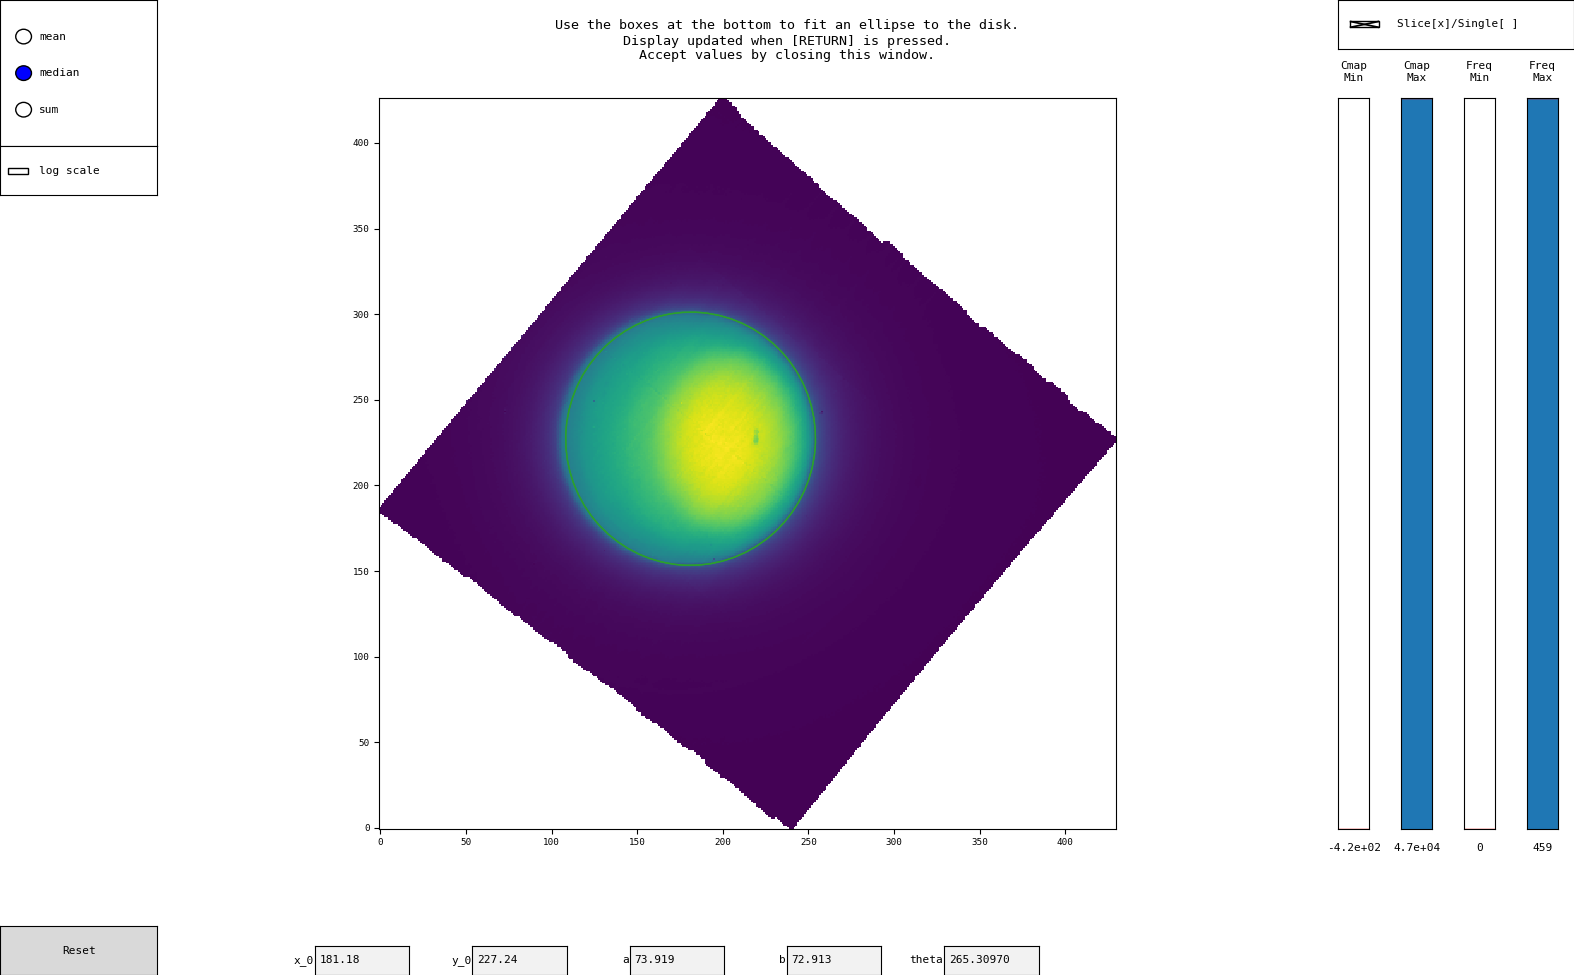
\includegraphics[width=\textwidth]{figures/fitscube_disk_finder.png}
	\caption{\textbf{Main Center Panel:} Shows the datacube with an ellipse (green, hard to see here) superimposed upon it. \textbf{Top Right:} Changes between multi and single channel mode, in multi-channel mode the image is a combination of all channels in the range as set by the selector in the top left. \textbf{Middle Right:} Colour map limits (Cmap Min, Cmap Max) and frequency channel limits (Freq Min, Freq Max). Clicking will set the relevant bar, values are shown at the bottom of the bars. Single-channel mode only shows a single frequency selector. \textbf{Top Left:} Aggregate selector swaps between combining channels via mean, median, or sum in multi-channel mode (unused in single-channel mode). Logarithmic scale can be toggled on or off. \textbf{Bottom Row:} `Reset' button resets all controls to their defaults. `x{\textunderscore}0' moves the ellipse center in the x-direction, `y{\textunderscore}0' moves the ellipse center in the y-direction. `a' changes the semi-major axis of the ellipse. `b' changes the semi-minor axis of the ellipse. `theta' rotates the ellipse. All numbers are given in pixels, fractions are possible. Close the dialog to accept the current values and continue with calculation.}
\label{fig:disk_fitter}
\end{figure}



\subsection{Webservices}

Located in \code{.../scripts/webservices}, there are two python files. \code{jplhorizons.py} has a couple of helper-functions based on `astroquery' to get ephemeris data from JPL-Horizons. \code{observatory_codes.py} holds routines that grab observatory codes from the internet and associate them with their names.


\subsection{Nemesis}

Located in \code{.../scripts/nemesis} most of these routines are superceeded by \textsc{nemesispy}. However, some of them may be useful and other scripts that interface with nemesis require them.


\subsection{fitscube/process}

Contains processing scripts for \textsc{sinfoni} data. Most of it is old and obsolete.

\subsection{astro{\textunderscore}resources.py}

\code{../scripts/astro_resources.py} contains some data about the physical parameters of planets. Used by the disk-fitting routines to get the sizes correct.

	%\bibliographystyle{abbrvnat}
	%\bibliographystyle{plain}
	\bibliographystyle{unsrtnat}
	\bibliography{references}

\end{document}
